\namedchapter[Daniel Łukwiński]{Stan aktualnej wiedzy}
Podstawową składową obrazu są piksele, czyli możliwie małe punkty jednakowej wielkości, posiadające jednolitą, określoną barwę. W pamięci komputera obrazy cyfrowe są zapisywane jako tablice, których każda komórka przechowuje informację o jednym pikselu. Tablicę taką można także przedstawić za pomocą funkcji:
\begin{equation}
	z = f(x,y), dla: x = 0, 1, 2, ..., N-1; y = 0, 1, 2, ..., M-1
   \label{funkcja_obrazu}
 \end{equation}
 gdzie:  
 \begin{equationDescriptor}
   \EQDitem{$N$}{szerokość obrazu,}
 	\EQDitem{$M$}{wysokość obrazu,}
 	 \EQDitem{$z$}{wartość funkcji w punkcie.}
 \end{equationDescriptor}
 
W najprostszym przypadku, dla obrazów czarno-białych, wartością wyrażaną przez tą funkcję jest stopień szarości każdego piksela. Obraz składa się wtedy z jednej, dwuwymiarowej tablicy o wymiarach $N$ na $M$.
W przypadku obrazów kolorowych do ich przedstawienia stosuje się kilka takich funkcji. Najpopularniejszym sposobem przedstawiania kolorów w grafice komputerowej jest model RGB. Skrót ten tworzą pierwsze litery angielskich nazw kolorów będących bazą w tym modelu: \textit{red} (czerwony), \textit{green} (zielony) oraz \textit{blue} (niebieski), których odpowiednia kombinacja umożliwia uzyskanie każdego koloru. W przypadku wykorzystania tego modelu obraz zapisany jest jako trzy tablice, przechowujące natężenia kolorów czerwonego, zielonego i niebieskiego. Przykład przedstawienia kolorowego obrazu za pomocą składowych R, G i B przedstawia ilustracja \ref{rgb}.

\begin{figure}[H]
\begin{center}
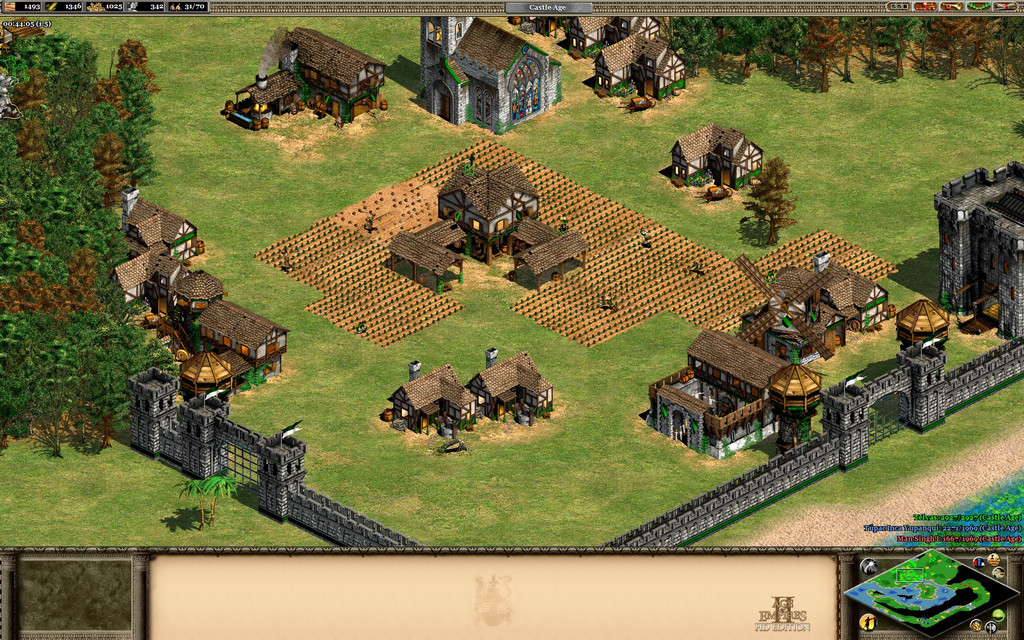
\includegraphics[scale=0.2]{imgs/rgb_all.jpg}
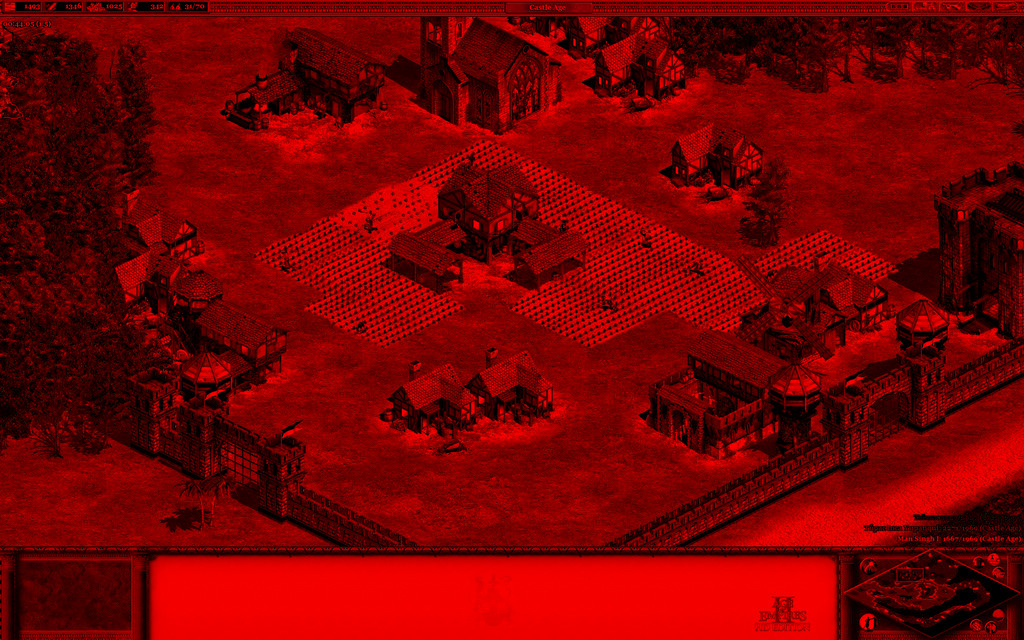
\includegraphics[scale=0.2]{imgs/red.jpg}
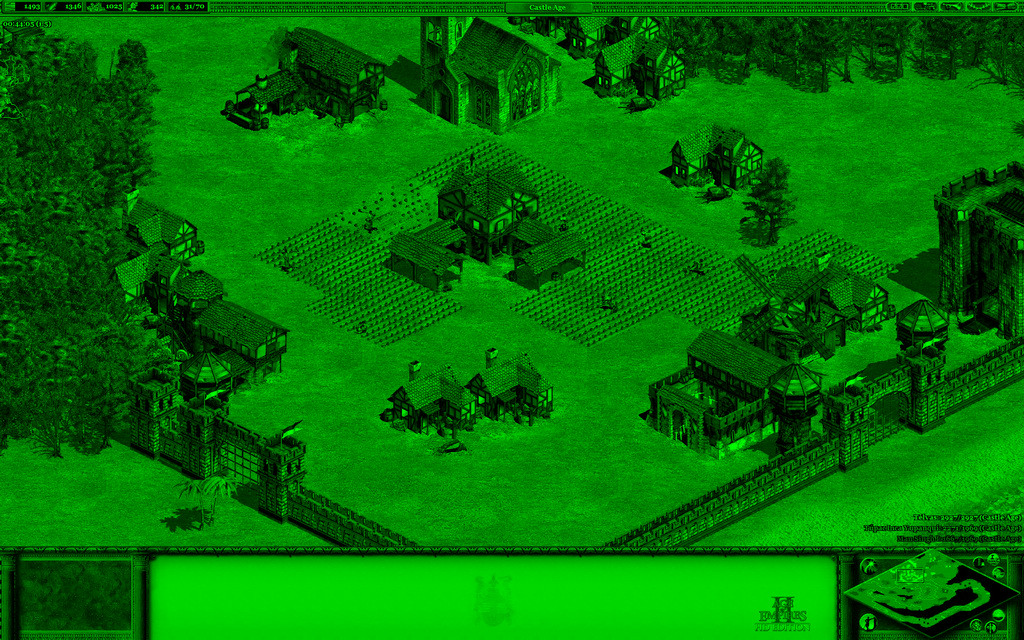
\includegraphics[scale=0.2]{imgs/green.jpg}
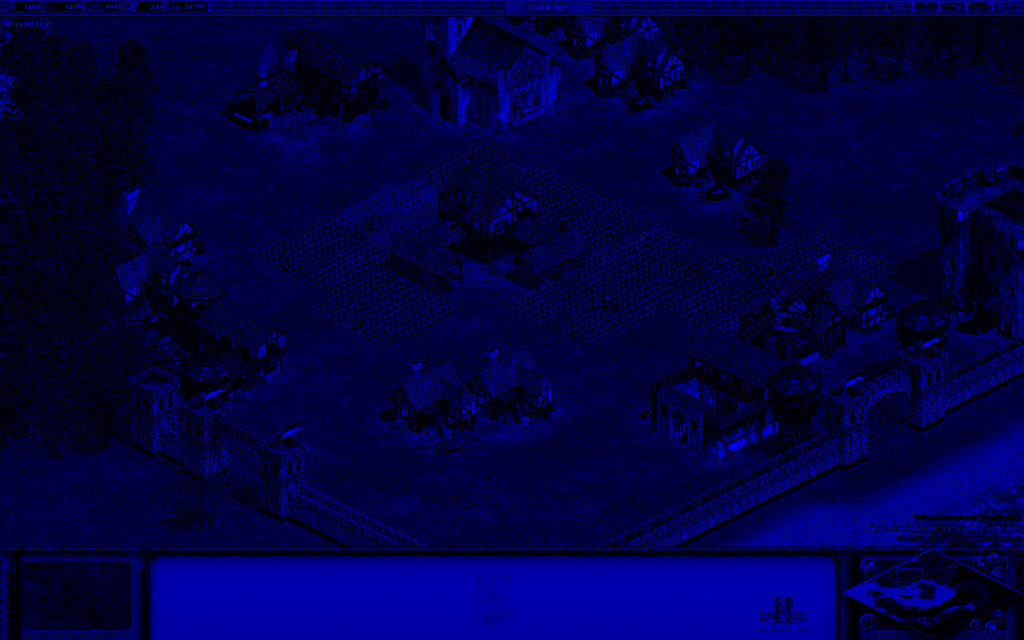
\includegraphics[scale=0.2]{imgs/blue.jpg}
\caption[Rozbicie obrazu kolorowego na RGB.]{\small{Ilustracja przedstawia oryginalny, kolorowy obraz oraz osobno jego trzy składowe, kolejno: czerwona, zielona i niebieska.}\footnotemark}
\label{rgb}
\end{center}
\end{figure}
\footnotetext{Zrzut ekranu z gry \emph{Age of Empires II}, przetworzenie obrazu wykonane przez autora za pomocą biblioteki \emph{OpenCV}.}

Obrazy, na których będą wykonywane operacje na potrzeby projektu, będą rejestrowane przez kamerę zamontowaną na robocie, a więc będą obrazami odzwierciedlającymi rzeczywiste otoczenie. Rejestracja rzeczywistego obrazu na postać cyfrową polega na dyskretyzacji obrazu oraz kwantyzacji jasności koloru\cite{Malina}. Kamera cyfrowa (lub aparat cyfrowy) jest urządzeniem pozwalającym na zarejestrowanie energii promieniowania elektromagnetycznego pochodzącego od obserwowanego obiektu. Przestrzenny rozkład energii jest rzutowany na dwuwymiarową płaszczyznę zbudowaną z elementów optoelektronicznych - matrycę. Powoduje to odłożenie się na każdym segmencie ładunku elektrycznego, którego wartość mierzymy, kwantujemy oraz zapisujemy w pamięci komputera. Wielkość matrycy oraz jej podzespołów decyduje o jakości wykonanego ,,pomiaru". W przypadku kolorowych obrazów rejestrowanie ich odbywa się poprzez jednoczesny pomiar trzech wartości, tzn. natężenia promieniowania fali o długości około 450 nm - kolor niebieski, 550 nm - zielony i 700 nm - czerwony. Jest to możliwe dzięki zastosowaniu odpowiednich filtrów pasmowoprzepustowych dla poszczególnych optoelementów matrycy.
Wynik tej operacji jest najczęściej zapisywany na 8 bitach - posiada wartość od 0 do 255 ($2^8$ daje 256 kombinacji). Pamiętając, że tworzone są trzy tablice, osobna dla każdego z kolorów RGB, dane każdego piksela zapisywane są na $3 \cdot 8 = 24$ bitach. Daje to kombinację $2^{24} = 16777216$ kolorów, czyli ilość przekraczającą już możliwości percepcji ludzkiego oka.

\namedsection{Analiza obrazu}

Obraz rzeczywistego otoczenia posiada dużą ilość informacji w znacznej mierze nadmiarowych, nie mających związku z poszukiwanym obiektem. Analizowanie obrazów dokonywane w ludzkim mózgu jest dla człowieka czynnością naturalną, ćwiczoną od chwili narodzin. Wydaje się więc być czymś prostym. W rzeczywistości próba powtórzenia tych procesów w sposób sztuczny jest rzeczą niezwykle trudną i złożoną. Cały proces wydobywania informacji z obrazu można podzielić na trzy etapy: przetwarzanie, analizę oraz rozpoznawanie.

Przetwarzanie obrazu to proces charakteryzujący się tym, że na jego wyjściu, tak samo jak na wejściu, znajduje się obraz cyfrowy. Operacje te wykonuje się w celu poprawy jakości obrazu lub uwypukleniu jego cech. Wymienione cele mogą iść w parze, np. w przypadku filtrów usuwających szumy lub wyostrzających krawędzie. Czasem jednak istnieje potrzeba takiego przetworzenia obrazu, które uwypukli pewne cechy lub dostosuje obraz od wymogów dalszej analizy. Przykładem może być ograniczenie palety kolorów. Obecnie znanych oraz stosowanych jest bardzo duża liczba różnego rodzaju metod przetwarzania obrazu. Niektóre z nich są uniwersalnymi, powszechnie stosowanymi metodami, wiele innych jednak dostosowane jest do pewnych bardzo sprecyzowanych zadań.

Obraz otoczenia rzeczywistego charakteryzuje się dużą nadmiarowością informacji. W celu ograniczenia ich tylko do tych potrzebnych w danym procesie stosuje się analizę obrazu, czyli inaczej wydobycie cech. W ten sposób można określić operacje, które wejściowy obraz zamieniają na szereg danych. Powstaje w ten sposób zbiór (wektor) charakterystycznych cech obrazu. Najmniejszy wektor cech może składać się z jednego tylko elementu. Każdy analizowany obraz jest oceniany pod określonym kątem. Wynik operacji zapisywany jest w postaci liczbowej, w odpowiednim miejscu wektora. Wartości całego wektora cech dla obrazu można przedstawić za pomocą punktu w przestrzeni (tzw. przestrzeń cech) o liczbie wymiarów równej liczbie elementów w wektorze cech.

Samo zadanie rozpoznawania obrazu jest już operacją wyłącznie na danych pozyskanych w trakcie analizy. W ogólności polega ono na rozpoznaniu przynależności różnego typu obiektów do pewnych klas abstrakcji\cite{Tadeusiewicz_flasinski}. Klasą abstrakcji nazywamy pewien zbiór obiektów mających wspólne cechy, a całą przestrzeń cech można podzielić na obszary odpowiadające konkretnym klasom. Klasy te mogą być tworzone na bieżąco, w oparciu o przyjmowane wartości cech lub ustalone z góry, na bazie pewnego zbioru danych uczących. Zbiorem uczącym z kolei nazywamy pewien zadany z góry ciąg obiektów, z których każdy posiada dwie zmienne: wektor wartości cech obrazu oraz oznaczenie klasy abstrakcji, do której należy\cite{Materka}. Za przydzielanie obrazu do jednej z klas abstrakcji odpowiada tzw. reguła decyzyjna, będąca algorytmem kierującym się pewnym określonymi wcześniej zasadami. Przykładowy problem stawiany przed tego typu algorytmem reprezentuje ilustracja \ref{zbior}. Przedstawia ona rozmieszczenie obiektów z dwóch klas abstrakcji pochodzących ze zbioru uczącego (czarne oraz białe koła), posiadających dwuelementowy wektor cech, których wartości reprezentowane są na osiach X oraz Y. Ostatni element, przedstawiony jako trójkąt, jest nowym obiektem, którego należy zakwalifikować do którejś z klas.

\begin{figure}[H]
\begin{center}
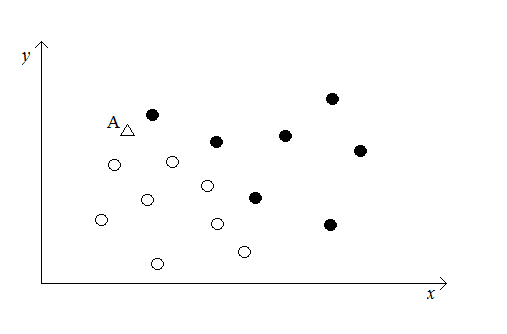
\includegraphics[scale=0.6]{imgs/hardtask2.png}
\caption[Przykładowe zadanie reguły decyzyjnej.]{\small{Ilustracja przykładowe zadanie stawiane przed regułą decyzyjną. Białe i czarne koła należą do dwóch klas zbioru uczącego, trójkąt \textit{A} jest badanym obiektem.}}
\label{zbior}
\end{center}
\end{figure}

Także w tym przypadku istnieje wiele metod, wykorzystywanych w algorytmach, reguły decyzyjnej. Najprostszymi są metody minimalnoodległościowe, w ogólności przyporządkowujące obiekt do tej klasy, do której należy ich najbliższy sąsiadujący obiekt. Wśród bardziej rozbudowanych technik możemy wyróżnić metodę funkcji potencjałowych. Polega ona na zdefiniowaniu funkcji potencjału dla każdego obiektu ze zbioru uczącego, a następnie zsumowaniu tych funkcji w ramach każdej klasy, tworząc tzw. funkcje przynależności. Klasyfikacji obiektu dokonuje się poprzez wyznaczenie funkcji przyjmującej największą wartość w punkcie, w którym znajduje się badany obiekt.
